\documentclass[11pt]{article}
\usepackage[a4paper, portrait, margin=1in]{geometry}
\usepackage{graphicx}
\usepackage{hyperref}
\usepackage{caption}
\usepackage[labelformat=simple]{subcaption}    %%Adding option to remove parenthesis
\renewcommand{\thesubfigure}{\normalsize Figure \thefigure. (\alph{subfigure}):}
% \usepackage{subcaption}
% \usepackage{subcaption}
%\usepackage{dirtytalk}
\usepackage{float}
\usepackage{eldar_report}
% Useful packages
\usepackage{amsmath}
% \newcommand\norm[1]{\lVert#1\rVert}
\newcommand\normx[1]{\Vert#1\Vert}
\usepackage{graphicx}
\usepackage{lifetime}
\newcommand{\Dana}[1]{\textcolor{purple}{\bf Dana: #1}}
\newcommand{\Julian}[1]{\textcolor{purple}{\bf Julian: #1}}


\begin{document}

\title{Robustness of Multi-Label Neural Networks}

\author{
    \textbf{Julian Mour} \\
    \\
    Advisor: Dana Drachsler Cohen\\
    Technion - Israel Institute of Technology
}

\maketitle

\section{Introduction}

In the last years, many works have demonstrated that deep neural networks (DNNs) are susceptible to a variety of adversarial example attacks, e.g.,~\cite{ref7,ref15,szegedy2014intriguing,ref17,ref29,ref56}.
Most adversarial attacks add small changes to the input that fool the network.
However, some attacks, known as $L_0$ attacks, focus on perturbing a very small number of pixels (e.g., one) to an arbitrary value~\cite{OnePixelAttack, alatalo2021chromatic, vargas2019understanding}.
This type of attack is very effective for concealing adversarial modification in practice, and it can provide geometrical theoretical insight into the input space of a classifier.
%Previous studies have shown that given an input image and a classifier (e.g. convolutional neural network), a perturbation of a single pixel or a very small and almost imperceptible perturbation of all pixels in the input image\cite{szegedy2014intriguing} can lead to misclassification.
%Examining different approaches for adversarial attacks may help network designers gain a deeper understanding of the vulnerabilities of their networks and then utilize that information to improve the network's robustness.\Dana{a bit general}
These attacks are usually local: for each input, they perform a computation to determine the perturbation, which may take a few minutes.
Furthermore, these attacks are not robust to input transformation, so each input must be processed differently.

In this thesis, we will design universal $L_0$ attacks, which rely on programs.
The key idea is that program can be specific to input but can be executed much faster and thus will be easier compared to prior attacks.
The program will determine which pixels to perturb and to which values. 
 %is to develop a framework for synthesizing universal adversarial programs. A program should, given an unknown input image, perturb a small number of pixels in order to carry out a successful untargeted attack. 
 Unlike previous adversarial attack methods, our programs do not employ independent optimization for each image but rather find structures/rules that can be applied to every new input to identify which pixels will be perturbed and how. 
 Our focus is on programs that have two stages.
 As the first stage, the goal is to limit the search space for a successful attack to a relatively small area in the input image.
 During the second stage, the focus is primarily on identifying the perturbation (its location and magnitude) within that small area.
 %We concentrate on programs that have conditions that are based on different areas of the input in order to determine the perturbation. We also examine programs that use neural networks to determine the location and magnitude of the perturbation.
 
 Our key idea is to formulate this problem as an optimization problem in which we try to find the optimal program.
 Two methods have been considered in terms of the initial stage of the program.
 First is an evaluation search that is trained on a limited set of inputs and given a set of possible program instructions.
 With each successive iteration, the search seeks to improve the program based on previously generated programs.
 In the second technique, a deep neural network is used to predict the locations and magnitudes of the perturbed pixels.
 For the second stage of the program, we developed a small program that iteratively examined all possibilities in a specific area.
 
 In our preliminary research, we implemented our optimization approach on CIFAR-10 dataset on ResNet-18~\cite{he2015deep} and evaluated it.
 We compared our results to the well-known \("\)one-pixel attack method\("\)~\cite{OnePixelAttack} which is our baseline.
 Our initial results indicate that our program generated attacks that had almost the same success rate as the baseline, but with much shorter execution times and significantly fewer queries.

In the future, we intend to improve our algorithms to ensure a greater success rate of the attacks and shorter execution times with fewer queries.
Additionally, we would like to leverage our programs to provide a better understanding of the network's decision boundaries and the factors that contribute to an attack's success.

\section{Problem Definition}
In this section, we define the problem we address.

Informally, we are interested in developing an efficient algorithm that given a single image, it returns a robust layer-neighborhood for a target object (target class);
A robust sequence of epsilons each representing the perturbation per layer.
Each layer is defined to be a set of pixels that share the same distance from a specific non-target object (non-target class) in the image.

Formally, Given a classifier $F$, an image $x$ of size $n\times m$ containing two objects: $c_{target}$ and $c_{non-target}$ \textrm{s.t.} $F(x)$ = \{$c_{target}$, $c_{non-target}$\},
we define the set of layers to be:
\begin{gather*}
    $ L_x = \{l_0^x, l_1^x, \ldots, l_r^x\}\\
    \textrm{s.t.} $ l_d^x = \{(i,j) \in $[1,n]\times [1,m]$ \mid dist((i, j), c_{non-target}) = d\}
\end{gather*}

We aim to build a program that returns a sequence of epsilons $(\varepsilon_0^x, \varepsilon_1^x, \ldots, \varepsilon_r^x)$ representing a robust perturbations of the pixels in the corresponding layers for the target class.
Formally:
\begin{gather*}
    $ \varepsilon_x = (\varepsilon_0^x, \varepsilon_1^x, \ldots, \varepsilon_r^x)\\
    \textrm{s.t.} $ \forall x' \in N(x): c_{target} \in F(x')\\
    N(x) = \{x' \mid \forall l_d^x\in L_x: \forall (i,j)\in l_d^x: x'_{i,j} \in [x_{i,j}-\varepsilon_d^x, x_{i,j}+\varepsilon_d^x]\}\\
\end{gather*}

\section{Our Approach}

In this thesis, we will build a program that given a multi-label classifier and an image, can find a layer-neighborhood of the image around a certain object (non-target class) that is robust for another object (target class) in the image.
A straight-forward solution would be to calculate each epsilon individually using a verifier and binary search.
Problem is this approach is very expensive in time hence inefficient.
Our approach aims to reach similar results as the straight-forward one, but in much less time.
In principle, our approach is similar to MaRVeL's~\cite{MARVEL}.
The desired program will have two main components:

\begin{itemize}
    \item The Verifier - The verifier's main job is to check whether a given layer-neighborhood of an image is robust for the classifier and pass the result to the optimizer.
    Since this is a multi-label classifier, we are interested only in the target class robustness;
    The verifier will say that the neighborhood is robust if and only if all images in the neighborhood are classified to the target class.
    The verifier in our case is a MILP based on the MIPVerify program~\cite{MIPVERIFY} that translates the robustness problem of a multi-label Neural-Network to a MILP maximization problem and uses the Gurobi Optimizer to solve it.
    In addition to checking whether the neighborhood is robust or not, the verifier returns the weakest points of the image.
    These are the points in the checked neighborhood that are least robust and the verifier will pass them to the optimizer as well.
    \item The Optimizer - The optimizer's job is to update a given robust layer-neighborhood by expanding it more, as we intend to maximize the norm of the neighborhood.
    In practice, we try to maximize the norm of the neighborhood and the Robustness Level (RL) of the classifier as well.
    This is done by computing the gradients of both components;
    The norm's gradient is computed in a straightforward way while the RL's gradient is computed using the weakest points found by the verifier.
    At last, we calculate the step gradient, which is a combination of both previous gradients, and expand the neighborhood towards the step gradient.
    If the neighborhood checked by the verifier isn't robust, then we skip the optimization part.
    Instead, we try to minimally shrink the neighborhood so that its robust.
    We do that in two different approaches:
    \begin{itemize}
        \item Fixed weights - We shrink the neighborhood using fixed weights, where we aim to shrink the neighborhood more in layers that are far from the non-target object and less in layers that are close to it.
        \item Sensitivity weights - Similar to the fixed weights approach, but we aim to shrink more in layers that are less sensitive to perturbations.
        We get the sensitivity weights of an image by using the Vanilla Gradient method, introduced by Simonyan et al.~\cite{VANILLAGRADIENT}
    \end{itemize}
    The new layer-neighborhood will be the input of the verifier in the next iteration.
\end{itemize}
Like that, we do this in iterations many times until convergence of the layer-neighborhood and the RL\@.
We aim to reach a maximal robust layer-neighborhood at the end of the process.


\section{Preliminary Results}
We implemented our approach and ran it on part of the DOUBLE-MNIST test dataset, consisting of images from ten classes (the 10 different digits), each image classified to two different classes (contains two different digits).
An example of a test dataset sample is shown in Figure~\ref{DOUBLE-MNIST sample}.
\begin{figure}
    \centering
    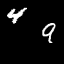
\includegraphics[width=0.4\textwidth]{3.png}
    \caption{DOUBLE-MNIST sample}
    \label{DOUBLE-MNIST sample}
\end{figure}

We ran our program on 3 different CNN multi-label DOUBLE-MNIST classifiers.
While the three of them solve the same classification problem, they differ in their training process:

\begin{itemize}
    \item Network with no defense - This network is trained regularly on the original DOUBLE-MNIST training dataset, without additional processing done to the training dataset.
    We present results of our program ran on this classifier and a single image, as a heatmap representing the epsilons per layer:
    \begin{figure}
         \centering
         \begin{subfigure}[b]{0.4\textwidth}
             \centering
             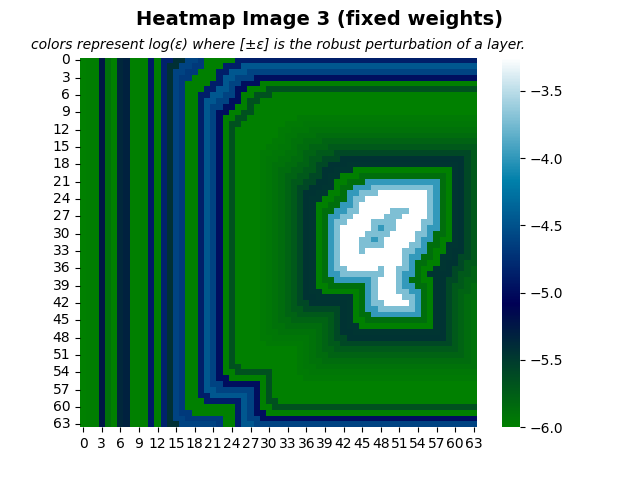
\includegraphics[width=\textwidth]{no_defense_fixed_weights.png}
             \caption{No defense, $FW$}
             \label{No defense, $FW$}
         \end{subfigure}
         \hfill
         \begin{subfigure}[b]{0.4\textwidth}
             \centering
             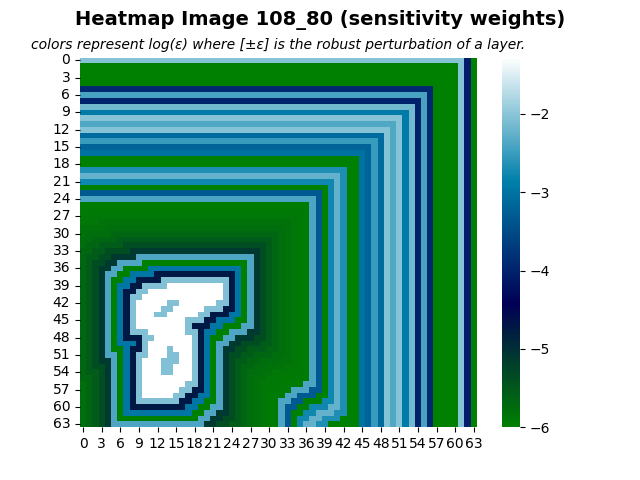
\includegraphics[width=\textwidth]{no_defense_sensitivity_weights.png}
             \caption{No defense, $SW$}
             \label{No defense, $SW$}
         \end{subfigure}
         \hfill
     \end{figure}
    \item Network with $L_0$ defense -
    \item Network with $L_{\inf}$ defense -
\end{itemize}


\section{Future Research Objectives}
In light of the preliminary work, we aim to further explore our ideas in the following directions:
\begin{itemize}
    \item Improved algorithm: success rate, execution times and number of queries - As a result of the current implementations and settings of our two approaches, the success rate of the attacks generated by the program is lower than our baseline.
    Therefore, we will implement different evolution methods, take a different approach to program instruction design, and develop a different architecture (e.g.\ transformers~\cite{vaswani2017attention}) for the deep network approach in order to increase success rates.
    While improving the success rate, we will strive to keep execution times as short as possible with a low number of queries.
    \item Explainability - One possible advantage of using a universal program to generate adversarial examples is to be able to explain the network's decision boundaries and the reasons that lead to the success of attacks.
    As an example, by synthesizing a program, we can determine which spatial regions or channels are relevant to the success of the attack.
    Using the deep learning approach, we are able to use other known tools for an explanation, such as LIME~\cite{ribeiro2016why}.
\end{itemize}

\section{Related Work}
Our thesis lies at the intersection of adversarial attacks and program synthesis. We next review some
related work.
\subsection{Adversarial Attacks}
Several aspects can be used to classify adversarial attacks~\cite{taxonomy}:
\begin{itemize}
    \item Targeted Vs. Untargeted - A targeted attack~\cite{papernot2015limitations} attempts to mislead a classifier by classifying input to a \textit{specific class} that differs from the true class of input.
    In untargeted attacks~\cite{ref7}, the goal is to cause the classifier to classify the input to \textit{any class} that is different from the true class.
    \item Individual Vs. Universal - Individual attacks generate different attacks for each different input, by optimizing the attack based on the input~\cite{ref7,papernot2015limitations,moosavidezfooli2016deepfool}.
    Universal attacks, on the other hand, generate one attack for all possible inputs.
    Studies from the last few years have indicated that universal adversarial attacks are capable of generalizing well to unseen data.
    The first method for universal adversarial attack was based on accumulating perturbations iteratively by composing perturbations for each data point~\cite{moosavidezfooli2017universal}.
    Other studies have used singular vectors~\cite{khrulkov2017art} and networks for adversary generation (NAGs)~\cite{mopuri2018nag}.
    \item White box Vs. Black box - In white box attacks, the architecture, weights, and parameters of the model are known to the adversary.
    First, white box adversarial attacks were derived through the generation of artificial perturbations using gradient-based optimization~\cite{szegedy2014intriguing}.
    There have been numerous works since then that have demonstrated different approaches to generating white-box adversarial attacks, such as FGSM\cite{ref7}, JSMA~\cite{papernot2015limitations}, and Deepfool~\cite{moosavidezfooli2016deepfool}.
    Attackers using black box methods assume they can only query the model without any further knowledge of it.
    Several studies have shown that a black-box approach can lead to generating successful attacks~\cite{BlackBox1, BlackBox2, BlackBox3, BlackBox4}.
\end{itemize}

Additionally, we investigate $L_0$ attacks, which aim to modify a small number of pixels.
In previous studies, it has been demonstrated that even a single pixel perturbation can lead to successful attacks\cite{OnePixelAttack, alatalo2021chromatic, vargas2019understanding}.

\subsection{Program synthesis}
Program synthesis is the task of automatically generating a computer program from user requirements.
It has been studied for decades and shown success in a variety of fields,
such as data wrangling\cite{inbook}, code repair\cite{d39antoni2016qlose}, code suggestions\cite{10.1145/2594291.2594321}, probabilistic modeling\cite{nori2015efficient} and superoptimization\cite{10.1145/36206.36194}.
Later, constructive techniques have been developed, such as enumerative
search\cite{6679385}, programming by examples\cite{inbook}, constraint solving\cite{CSP}, stochastic search\cite{schkufza2012stochastic}, neural program synthesis\cite{parisotto2016neurosymbolic} and genetic programming\cite{Koza92}.
In our preliminary work, we focused on a variant of genetic search.



\bibliography{bibliography}
\bibliographystyle{plain}

\end{document}
